\section{Paper 7}
\subsection{\emph{"Variational-Based Mixed Noise Removal With CNN Deep Learning Regularization"}}

\begin{frame}{INTRODUCTION}
    Random noise distributions correspond to standard probabilistic distributions, 
    such as the Gaussian, Poisson and other distributions. There have 
    been many methods that attempt to clean up noisy images. Other tools such as the Variational method have been widely used. 
    This method is based on reducing the cost function containing the fidelity 
    term of the data, useful for calculating the difference between true and observed 
    data, and the regularization terms. In the 
    proposed article, the EM (Expectation-Maximization) algorithm is used to 
    remove the noise, with the integration of a CNN process as regularization, 
    in order to create a new variational method.
\end{frame}

\begin{frame}{RELATED WORK - What types of image noises?}
    The noises analyzed in this paper are mainly two categories of Gaussian 
    noises:
    \begin{minipage}{\linewidth}
        \centering
        \begin{minipage}{0.45\linewidth}
            \begin{block}{GAUSSIAN MIXED-NOISE}
                $$
                \small
                n = \left\{
                    \begin{array}{cc}
                        n_1, & with~probability~r_1\\
                        n_2, & with~probability~r_2\\
                        \cdots, & \cdots\\
                        n_k, & with~probability~r_k\\ 
                    \end{array}
                    \right\}
                $$
            \end{block}  
        \end{minipage}
        \hspace{0.05\linewidth}
        \begin{minipage}{0.47\linewidth}
            \begin{block}{GAUSSIAN RANDOM NOISE}
                $$
                \small
                n = \left\{
                    \begin{array}{cc}
                        n_1, & with~probability~1-r\\
                        n_2, & with~probability~r\\
                    \end{array}
                    \right\}
                $$
            \end{block} 
        \end{minipage}
    \end{minipage}
    where $ n_k $ is the \emph{k}-th noise component with probability density function (PDF) 
    $ p_k $ and $ r_k $ are the unknown mixture ratios and their sum is equal to 
    1. Each type of noise has a standard deviation ($\sigma$) which indicates the 
    amount of noise distribution present.     
\end{frame}

\begin{frame}{RELATED WORK - Variational Method Approach}
    To obtain the clean image is necessry minimizing a cost functional(\ref{cost}).
    \begin{block}{COST-FUNCTIONAL}
        \begin{equation}\label{cost}
            F(u) = E(u)+\lambda\mathcal{J}(u)
        \end{equation}
    \end{block}
    where $E(u)$ is the set of data fidelity terms belonging to each pixel of the 
    image $u$ useful to measure the discrepancy between the true and the 
    observed data and it can derived from the maximum likelihood estimation 
    of noise, task perfromed by the EM algorithm \footfullcite{0884882814}.  $\mathcal{J}$ is a regularizer while $ \lambda $ 
    control the balance of the terms
\end{frame}

\begin{frame}{RELATED WORK - EM Algorithm (An Optimization problem)}
    The EM algorithm is applied to this noise which has the task of estimating the noise 
    and classifying it by minimizing the terms of \ref{HFunction}. The minimization of each 
    weight $w$ leads to a continuous updating of this parameter which translates 
    into greater precision in determining the noise on each individual pixel.
    \begin{equation}\label{HFunction}
        (u^*, \Theta^*, w^*) = \argmin_x\left\{H(u,\Theta,w) + \lambda_1\mathcal{J}(u)\right\}
    \end{equation}
    where $\Theta^*$ is a statistical parameters set contains noise parameters such as mixture ratios ($r$), means and variances ($\sigma^2$).
\end{frame}

\begin{frame}{THE PROPOSED METHOD (EM-CNN) - Architecture}
    \begin{minipage}{\linewidth}
        \centering
        \begin{minipage}{0.45\linewidth}
            The convolutional neural network (CNN) performs the following tasks            
            \begin{enumerate}
                \item Smoothness (Denoiser)
                \item Regularization (TV)
                \item Synthesis (Best Choice)
                \item Parameters estimation (EM)
                \item Noise classification (EM)
                \item Output (Restored image and Noise Estimation)
            \end{enumerate} 
        \end{minipage}
        \hspace{0.05\linewidth}
        \begin{minipage}{0.47\linewidth}
            \begin{figure}[h!]
                \centering
                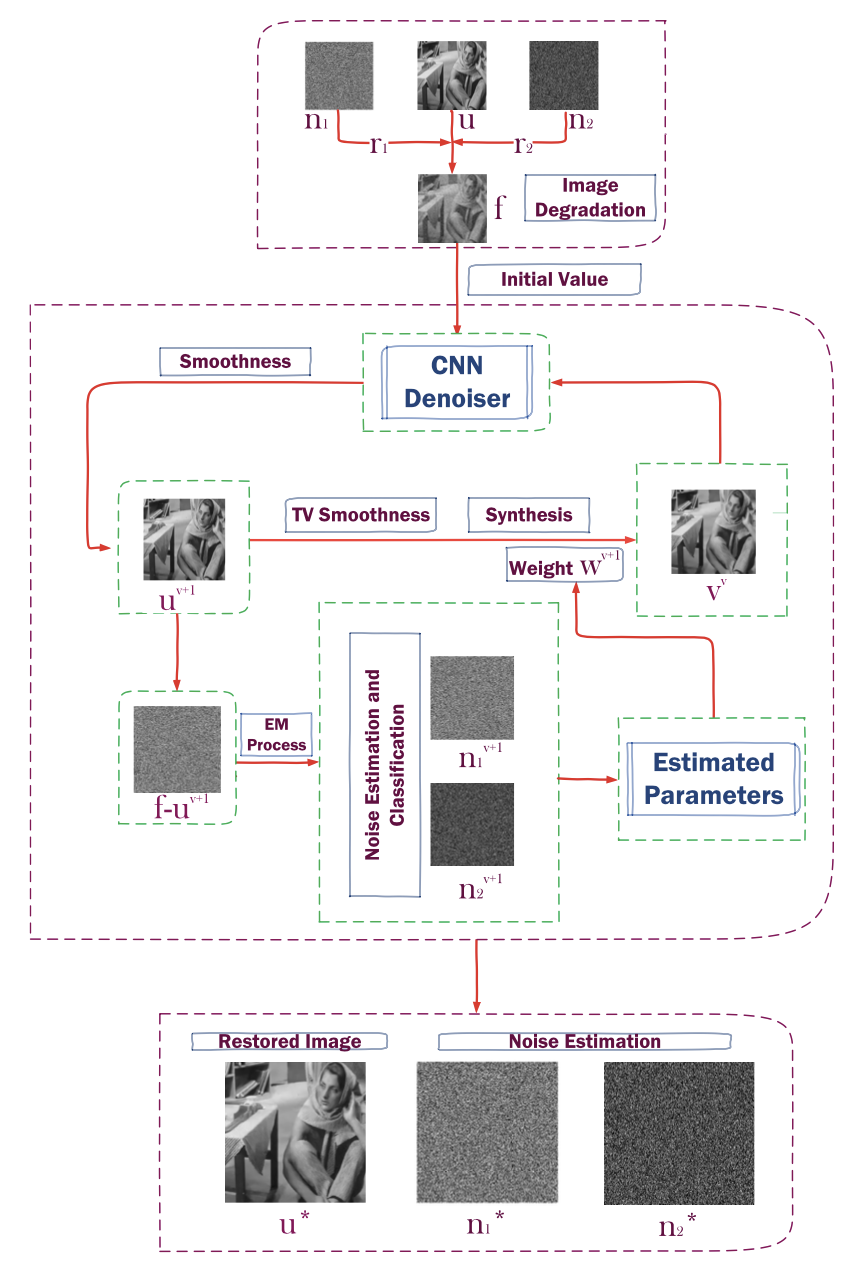
\includegraphics[width = 1 \linewidth]{images/paper7/flowchart.png}
                \centering
                \label{fig:EM-CNN}
            \end{figure}
        \end{minipage}
    \end{minipage}
\end{frame}

\begin{frame}{EXPERIMENTAL RESULTS - Gaussian mixed-noise}
    The indexs used to estimate the quality of the restructured images are 
    the \emph{Signal-to-Noise Ratio} (PSNR) and the \emph{Structural Similarity Index} 
    (SSIM). The results obtained by comparing different methods with the 
    proposed, in image reconstruction and Gaussian mixed-noise removal, one 
    are visible in figure \ref{fig:GMNComp} and table \ref{indexCompare}. The test set images were taken from 
    the BSDS100 dataset.
    \begin{figure}[h!]
        \centering
        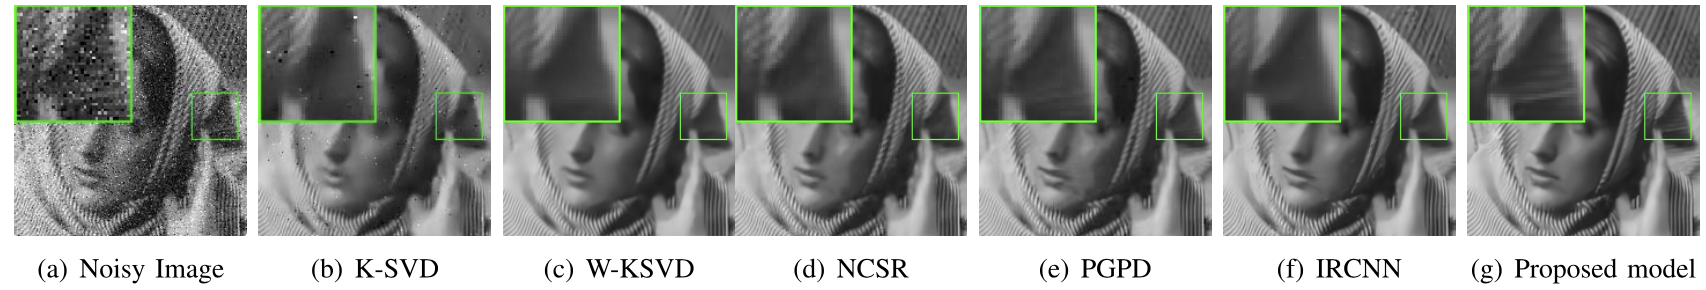
\includegraphics[width = 0.8\linewidth]{images/paper7/GMN comparison.png}
        \centering
        \caption{Image reconstruction under Gaussain mixture noise comparison.}
        \label{fig:GMNComp}
    \end{figure}
     
    \begin{table}[htbp]
        \centering
        \begin{adjustbox}{width=0.8\textwidth}
        \begin{tabular}{|c||ccc|ccc|ccc|}
            \hline
                & \multicolumn{3}{c||}{$\sigma_1=5 ~~~\sigma_2=30 $} & \multicolumn{3}{c||}{$\sigma_1=10 ~~~\sigma_2=50 $} & \multicolumn{3}{c||}{$\sigma_1=15 ~~~\sigma_2=75 $}\\
            \hline        
            $r_1:r_2\rightarrow$ & 0.3:0.7 & 0.5:0.5 & 0.7:0.3 & 0.3:0.7 & 0.5:0.5 & 0.7:0.3 & 0.3:0.7 & 0.5:0.5 & 0.7:0.3\\
            \hline 
            \hline
            \multirow{2}{*}{PGPD\cite{0884882815}} & 29.42 & 30.16 & 31.19 & 27.23 & 27.88 & 28.78 &25.64 & 26.26 & 27.14\\
            & 0.8132 & 0.8349 & 0.8544 & 0.7404 & 0.7634 & 0.7874 & 0.6790 & 0.7044 & 0.7336\\
            \hline
            \multirow{2}{*}{IRCNN\cite{0884882819}} & 29.83 & 30.53 & 31.48 & 27.66 & 28.25 & 29.04 & 19.37 & 25.22 & 27.32\\
            & 0.8262 & 0.8451 & 0.8664 & 0.7611 & 0.7789 & 0.7993 & 0.2948 & 0.6423 & 0.7426\\
            \hline
            \multirow{2}{*}{Proposed} & \bfseries{29.88} & \bfseries{31.26} & \bfseries{32.72} & \bfseries{28.01} & \bfseries{29.00} & \bfseries{30.37} & \bfseries{26.23} & \bfseries{27.41} & \bfseries{28.84}\\
            & \bfseries{0.8273} & \bfseries{0.8785} & \bfseries{0.9094} & \bfseries{0.7801} & \bfseries{0.8112} & \bfseries{0.8528} & \bfseries{0.6931} & \bfseries{0.7613} & \bfseries{0.8077}\\
            \hline
        \end{tabular}
        \end{adjustbox}
        \caption{Average PSNR and SSIM values on BSD100 datasets of some methods.}
        \label{indexCompare}
    \end{table}
    
\end{frame}

\begin{frame}{EXPERIMENTAL RESULTS - Gaussian random-noise}
    As for the reconstruction of an image affected by random noise, also 
    called salt and pepper noise, the results obtained from the comparison of 
    different methods are visible in figure \ref{fig:saltComp} and in table \ref{GNPINIndex}. As in the previous 
    experiment, the indexs are calculated by changing the mixed-ratio $r$ and 
    standard deviation $\sigma$ values.
    \begin{figure}[h!]
        \centering
        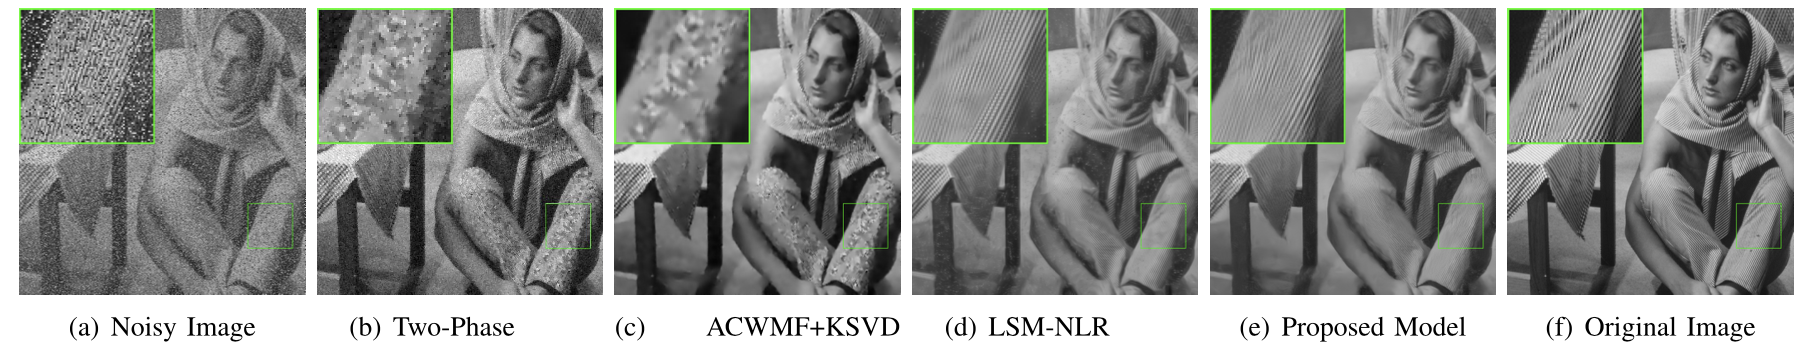
\includegraphics[width = 0.7\linewidth]{images/paper7/salt.png}
        \centering
        \caption{Image reconstruction under Gaussain noise plus random-valued noise comparison.}
        \label{fig:saltComp}
    \end{figure}
    
    \begin{table}[h!]
        \centering
        \begin{adjustbox}{max width=0.7\textwidth}
        \begin{tabular}{|c||ccc|ccc|ccc|}
            \hline
                & \multicolumn{3}{c||}{$\sigma_1=5$} & \multicolumn{3}{c||}{$\sigma_1=10$} & \multicolumn{3}{c||}{$\sigma_1=15$}\\
            \hline        
            $r\rightarrow$ & 0.1 & 0.2 & 0.3 & 0.1 & 0.2 & 0.3 & 0.1 & 0.2 & 0.3\\
            \hline 
            \hline
            \multirow{2}{*}{Noisy} & 18.76 & 15.76 & 14.04 & 18.43 & 15.61 & 13.95 & 17.94 & 15.38 & 13.81\\
            & 0.3545 & 0.2290 & 0.1662 & 0.3313 & 0.2216 & 0.1626 & 0.3040 & 0.2109 & 0.1571\\
            \hline
            \multirow{2}{*}{Two-phase\cite{0884882828}} & 25.40 & 24.77 & 24.13 & 24.34 & 23.94 & 23.45 & 23.32 & 23.02 & 22.67\\
            & 0.6599 & 0.6313 & 0.5957 & 0.5116 & 0.4914 & 0.4655 & 0.4224 & 0.4058 & 0.3854\\
            \hline
            \multirow{2}{*}{ACWMF+K-SVD \cite{0884882844}\cite{0884882813}} & 26.07 & 25.27 & 24.54 & 25.50 & 24.91 & 23.13 & 24.64 & 24.19 & 23.67\\
            & 0.7130 & 0.6761 & 0.6333 & 0.5902 & 0.5613 & 0.5291 & 0.4855 & 0.4625 & 0.4414\\
            \hline    
            \multirow{2}{*}{LSM-NLR \cite{0884882826}} & 29.48 & 26.97 & 24.55 & 29.43 & 27.08 & 24.43 & 28.51 & 26.06 & 23.98\\
            & 0.6548 & 0.5774 & 0.4982 & 0.6420 & 0.5646 & 0.4770 & 0.6282 & 0.5458 & 0.4643\\
            \hline
            \multirow{2}{*}{$l_1-l_0$\cite{0884882829}} & 30.45 & 27.75 & 25.95 & 28.45 & 26.59 & 25.34 & 27.33 & 25.69 & 24.55\\
            & 0.8962 & 0.7911 & 0.7312 & 0.7539 & 0.6748 & 0.6293 & 0.6793 & 0.6010 & 0.5744\\
            \hline
            \multirow{2}{*}{Proposed} & \bfseries{31.06} & \bfseries{30.44} & \bfseries{27.66} & \bfseries{30.97} & \bfseries{29.5} & \bfseries{27.41} & \bfseries{29.74} & \bfseries{28.09} & \bfseries{25.73}\\
            & \bfseries{0.9214} & \bfseries{0.9157} & \bfseries{0.8497} & \bfseries{0.8943} & \bfseries{0.8749} & \bfseries{0.8316} & \bfseries{0.8530} & \bfseries{0.8222} & \bfseries{0.7750}\\
            \hline
        \end{tabular}
        \end{adjustbox}
        \caption{Average PSNR and SSIM values on one image of some methods.}
        \label{GNPINIndex}
    \end{table}
\end{frame}

\begin{frame}{CONCLUSION}
    Even reaching good performances, the proposed method does not always 
    manage to obtain better results than those of competing methods. 
    However, the average of the PSNR index achieved is the highest (Fig. \ref{fig:cropRes}).
    \begin{figure}[h!]
        \centering
        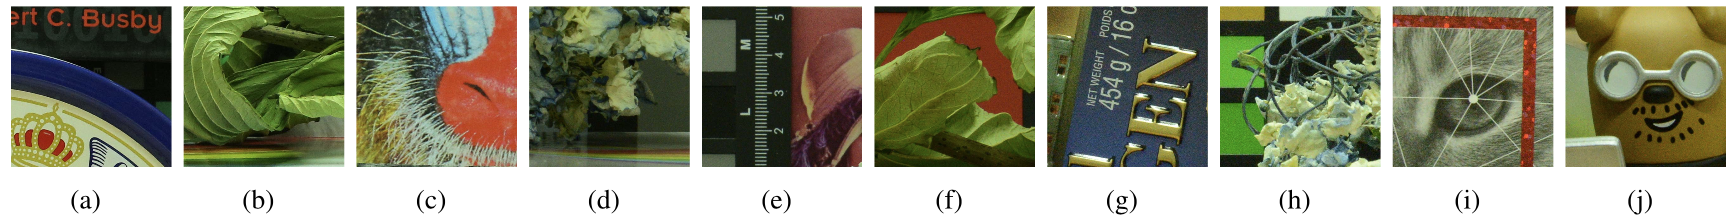
\includegraphics[width = \linewidth]{images/paper7/crop.png}
        \centering
        \caption{Cropped real noisy images.}
        \label{fig:crop}
    \end{figure}
    
    \begin{figure}[h!]
        \centering
        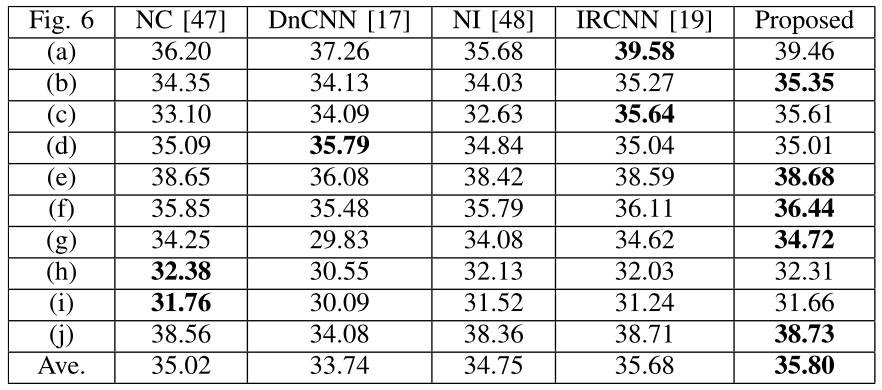
\includegraphics[width = 0.6\linewidth]{images/paper7/crop result.png}
        \centering
        \caption{PSNR result of different methods on cropped real noisy images.}
        \label{fig:cropRes}
    \end{figure}
    
\end{frame}

